%!TEX root = ../../PhD_thesis__Edouard_Leurent.tex

\graphicspath{{2-Chapters/2-Chapter/}}

\chapter{Literature Review}
\label{chapter:2}

\begin{flushright}
	\begin{tabular}{@{}l@{}}
		\emph{Souhaite que la route soit longue. [\dots]}\\
		\emph{Visite aussi beaucoup de villes égyptiennes,}\\
		\emph{et n’aie de cesse de t’instruire auprès de ceux qui savent.}\\
	\end{tabular}
	
	Konstantinos Kavafis, \href{https://eleurent.github.io/sisyphe/texts/ithaki.html}{\emph{Ithaque}}.
\end{flushright}

\abstractStartChapter{}%
This chapter provides an overview of the sequential decision-making literature in the specific context of Autonomous Driving. It is meant to summarise the main directions that researchers have taken to tackle this wide problem, and discuss the questions that one practitioner may ask themselves when trying to apply \acl*{RL} to \acl*{AD}. Thus, I will prioritise breadth rather than depth, and remind the reader that each of these sections is not comprehensive and has been surveyed independently.
\minitocStartChapter{}

\section{Sequential decision-making}
\label{sec:sequential-decision-making}

\Cref{sec:scopes-and-challenges} presented the \acl*{RL} framework, that formulates the learning procedure as an optimal control problem. In this section, I start by recalling other design principles that have been considered for coming up with a good driving policy $\pi$.

\subsection{Motion Planning}

The development of motion planning techniques for intelligent vehicles dates back to the late 80s, supported by international research projects such as Eureka (1987) of the Prometheus program, followed by the DARPA Grand and Urban Challenges (2004, 2007), and more recently the VIAC (2010), GCDC (2011) and Delphi (2015) challenges. In two surveys \citep{Gonzalez2016,Paden2016} studying the literature of this period, three main approaches have been identified.

\paragraph{Search-based algorithms}

This method is based on a regular discrete partition of the state space $\cS$ called a \emph{lattice}, which must be connected by feasible trajectories \citep[\eg][]{Pivtoraiko2005}. This framing reduces motion planning to the problem of finding a shortest path in a known graph. Then, traditional graph-search algorithms such as Dijkstra's algorithm \citep{Dijkstra1959}, $A^\star$ \citep{Hart1968} or $D^\star$ \citep{Stentz1994} can been used to compute the optimal trajectory. This technique has been applied by at least five different teams during the DARPA Urban Challenge for driving on structured roads and unstructured parking: Dijkstra for team Ben Franklin \citep{Bohren2008} and VictorTango \citep{Bacha2008}, and $A^\star$ for Stanford University \citep{Montemerlo2008} and KIT \citep{Kammel2008}, and $D^\star$ by the winning team from CMU \citep{Urmson2008}. Kinematics constraints can also be included in the configuration graph, as in \citep[\eg][]{Latombe1991,Fraichard1993,Laumond1994}.

\begin{figure}[tp]
	\centering
	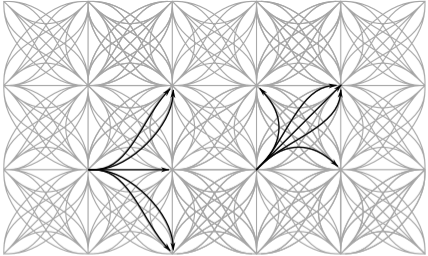
\includegraphics[width=0.5\linewidth]{img/lattice2}
	\caption{A lattice structure connects a discrete set of states by feasible trajectories}
\end{figure}

\paragraph{Sampling-based algorithms}

The limitation of search-based algorithms lies in the difficulty of formulating a regular lattice structure covering the states space $\cS$ with feasible transitions, and in the real-time constraint that may not be met by graph-search algorithms. To address them, sampling-based motion planners iteratively grow a set of reachable configurations by randomly sampling valid transitions. The most popular ones are \ac{PRM} \citep{Kavraki1996}, \ac{RRT} \citep{Lavalle98,Karaman2011} and \ac{MCTS} algorithms \citep{Coulom2006, Kocsis2006}. These methods have been used in the context of \acl*{AD} in \citep[\eg][]{Lamiraux2001,Sanchez2002,Lenz2016,Paxton2017,Faust2018}.

\paragraph{Optimisation-based algorithms}

The third approach consists in optimizing a parametrized trajectory with respect to a real-valued objective function. The most popular instance is interpolation between the current and goal states, which has been applied to various classes of functions in the context of Autonomous Driving, such as lines and circles \citep{Reeds1990}, clothoids \citep{Funke2012}, polynomials \citep{Xu2012}, and Bézier curves \citep{Gonzalez2016}.

These three approaches to motion planning thus rely on deterministic models of the vehicle dynamics. These models are often required to take a simple form so that the search or optimisation procedure can be solved efficiently, and other objects in the scene are often considered as static. In order to study more complex multi-agent interactions specifically, a collaborative approach to motion planning has been developed.

\paragraph{Cooperative planning}

The difficulty of predicting complex interaction patterns between multiple agents can be bypassed in one particular setting: cooperative motion planning for multiple vehicles. Indeed, the task of predicting how vehicles react to one another is replaced by the task of optimising the joint behaviour of all agents in the scene. As an effect, prediction outputs are replaced by input variables that can be chosen freely to maximise an objective function. Two main variations have been studied: coordination along fixed paths \citep{Altche2016,Altche2016b,Altche2017}, and general unconstrained motion planning \citep{LaValle1998}.
However, this framework does not allow to represent human behaviours, or more generally any behaviour that is not explained by the objective function. In particular, that lack of communication between agents and the resulting uncertainty lead to suboptimal, uncertain and multimodal trajectories that are not handled by cooperative planning approaches.


\subsection{Imitation Learning}
\label{sec:imitation-learning}

An orthogonal strategy to motion planning techniques is to learn a reactive policy $\pi(a|s)$ under supervision of an expert $\pi_E$ that produces a dataset $\cD$ of demonstration trajectories. To that end, a parametrized policy $\pi_\theta$ is optimised to minimise a regression loss $\cL$, for instance the $KL$ divergence to the expert actions distribution:
\begin{equation*}
\min_\theta \expectedvalue_{s\sim \cD} \left[\cL\left(\pi_{\theta}(a|s), \pi_E(a|s)\right)\right]
\end{equation*}
This approach is also referred to as behavioural cloning, and is particularly suited when only low-level high-dimensional inputs are available, such as camera images, which prevents access to the dynamics model required by motion planning approaches. 
The first application of imitation learning to autonomous driving is the ALVINN (Autonomous Land Vehicle In a Neural Network) project \citep{Pomerleau89}, where a 3-layer neural network was trained for the task of road following, as shown in \Cref{fig:alvinn}.
\begin{figure}[th]
	\centering
	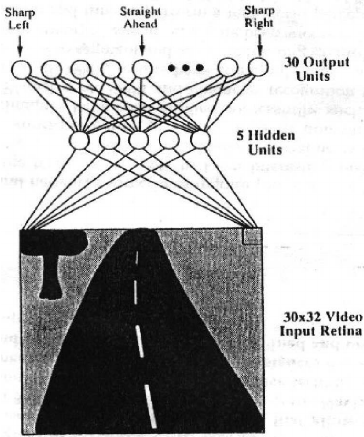
\includegraphics[width=0.4\linewidth]{img/alvinn}
	\caption{The 3-layer architecture used in ALVINN \citep{Pomerleau89}.}
	\label{fig:alvinn}
\end{figure}

\paragraph{Compounding errors} Unfortunately, the behavioural cloning paradigm is known to suffer from \emph{compounding errors}: since the future states depend on previous predictions (actions), the \iid assumption made in statistical learning does not hold. Therefore, small mistakes will place the system into states that are outside the training data distribution, as illustrated in \Cref{fig:compounding}, and resulting policies struggle to maintain high performances on long time horizons. This effect was identified and tackled in \citep{Ross2011}, who proposed to iteratively request expert labels (actions) from the states encountered by the current trained policy, rather than from the initial expert distribution. However, this can only be accomplished at the cost of a significant labelling effort. 
\begin{figure}[th]
	\centering
	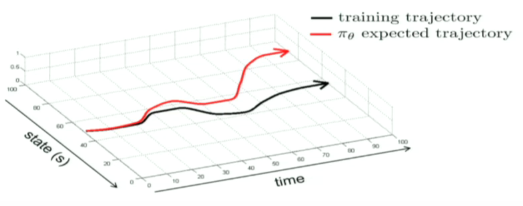
\includegraphics[width=0.7\linewidth]{img/cp4}
	\caption{As the agent deviates from the expert trajectories, the errors compound and push the agent further and further from the training distribution.}
	\label{fig:compounding}
\end{figure}
In the context of a Lane Keeping application, \citet{Bojarski2016} proposed instead to mitigate this issue during the data collection step by simulating deviations from the expert trajectories by means of two side cameras facing at the edge of the road. The corresponding synthetic expert controls were obtained by adding a constant adjustment term steer the vehicle back on track. The effect of compounding errors can also be delayed by further increasing the prediction performance, \eg by considering temporal dependencies as in \citep{Eraqi2017,Xu2017}. Other techniques than maximum likelihood estimation can be used to train the models, such as Generative Adversarial Imitation Learning \citep{Ho2016}, used for highway driving from range measurements in \citep{Kuefler2017,Bhattacharyya2018}.

\paragraph{Policy conditioning} A limitation of imitation learning for autonomous driving is fact that simply imitating human drivers by sampling likely trajectories is not sufficient: the sampling must also be conditioned on the current short-term destination specified by the Route planner. \citep{Codevilla2018} propose to achieve this by considering several policy heads for three possible behaviours when reaching an intersection: go straight, turn left or turn right. At test time, the appropriate policy is used at each intersection depending on the planned route. \citep{Rhinehart2020} present a more general approach that consists in learning a probabilistic model $q(s)$ of expert trajectories used as a prior, and inferring the maximum a posteriori trajectory given a test-time goal likelihood $p\parentheses{goal\mid s}$.

\subsection{Reinforcement Learning}

While the \ac*{MDP} framework undoubtedly constitutes a convenient theoretical framework for analysis, it may be too narrow a frame to accommodate the real world. In the sequel, by trying to cast the problem of Autonomous Driving as an \ac*{MDP}, we will identify multiple underlying assumptions that do not hold in practice, and relate them to existing research areas for which researchers proposed variants and solutions.

\section{States and partial observability}
\label{sec:partial-observability}

\begin{figure}[th]
	\centering
	\begin{subfigure}[b]{.7\linewidth}
		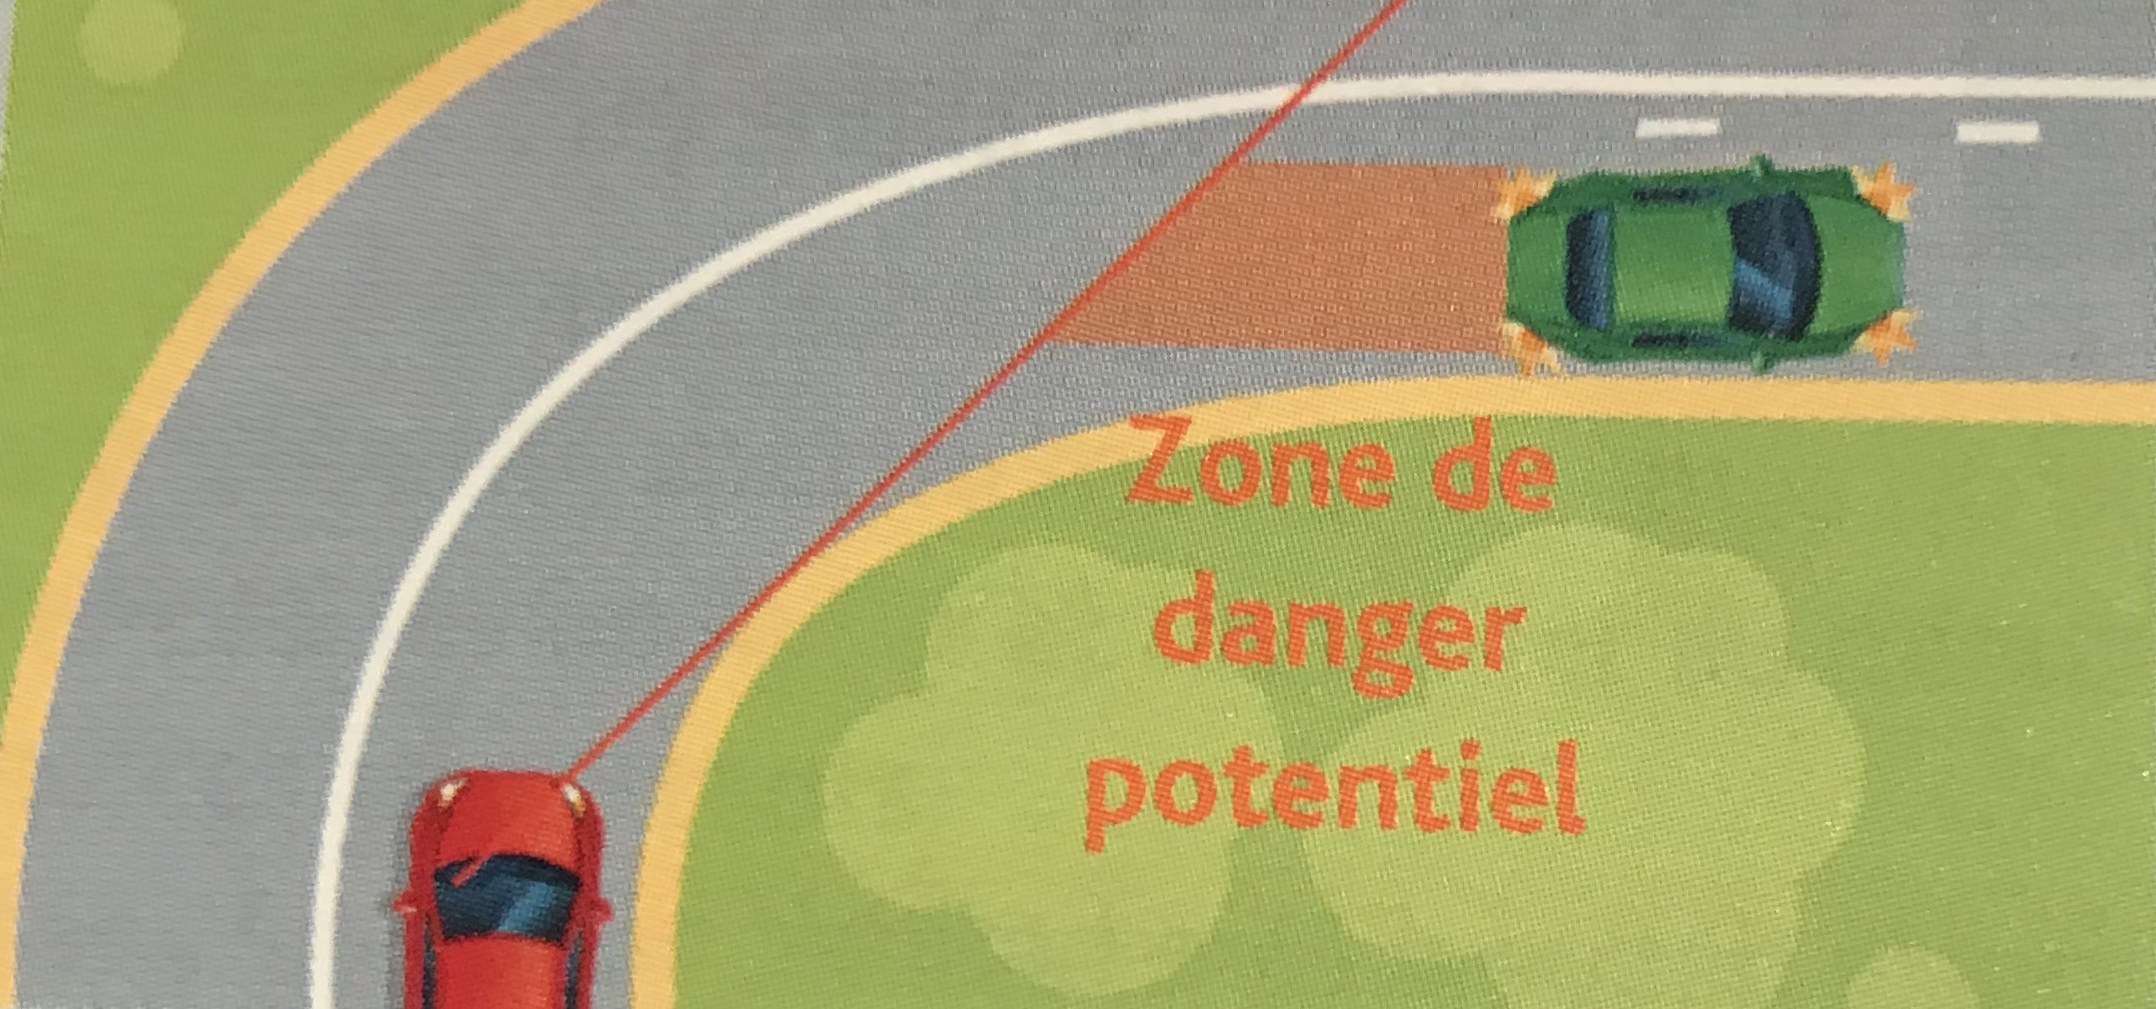
\includegraphics[width=\linewidth]{img/po-sensors}
		\caption{"Area of potential danger". A partial observability stemming from sensor occlusion in a turn.}
		\label{fig:po-occlusion}
	\end{subfigure}
	\begin{subfigure}[b]{.4\linewidth}
		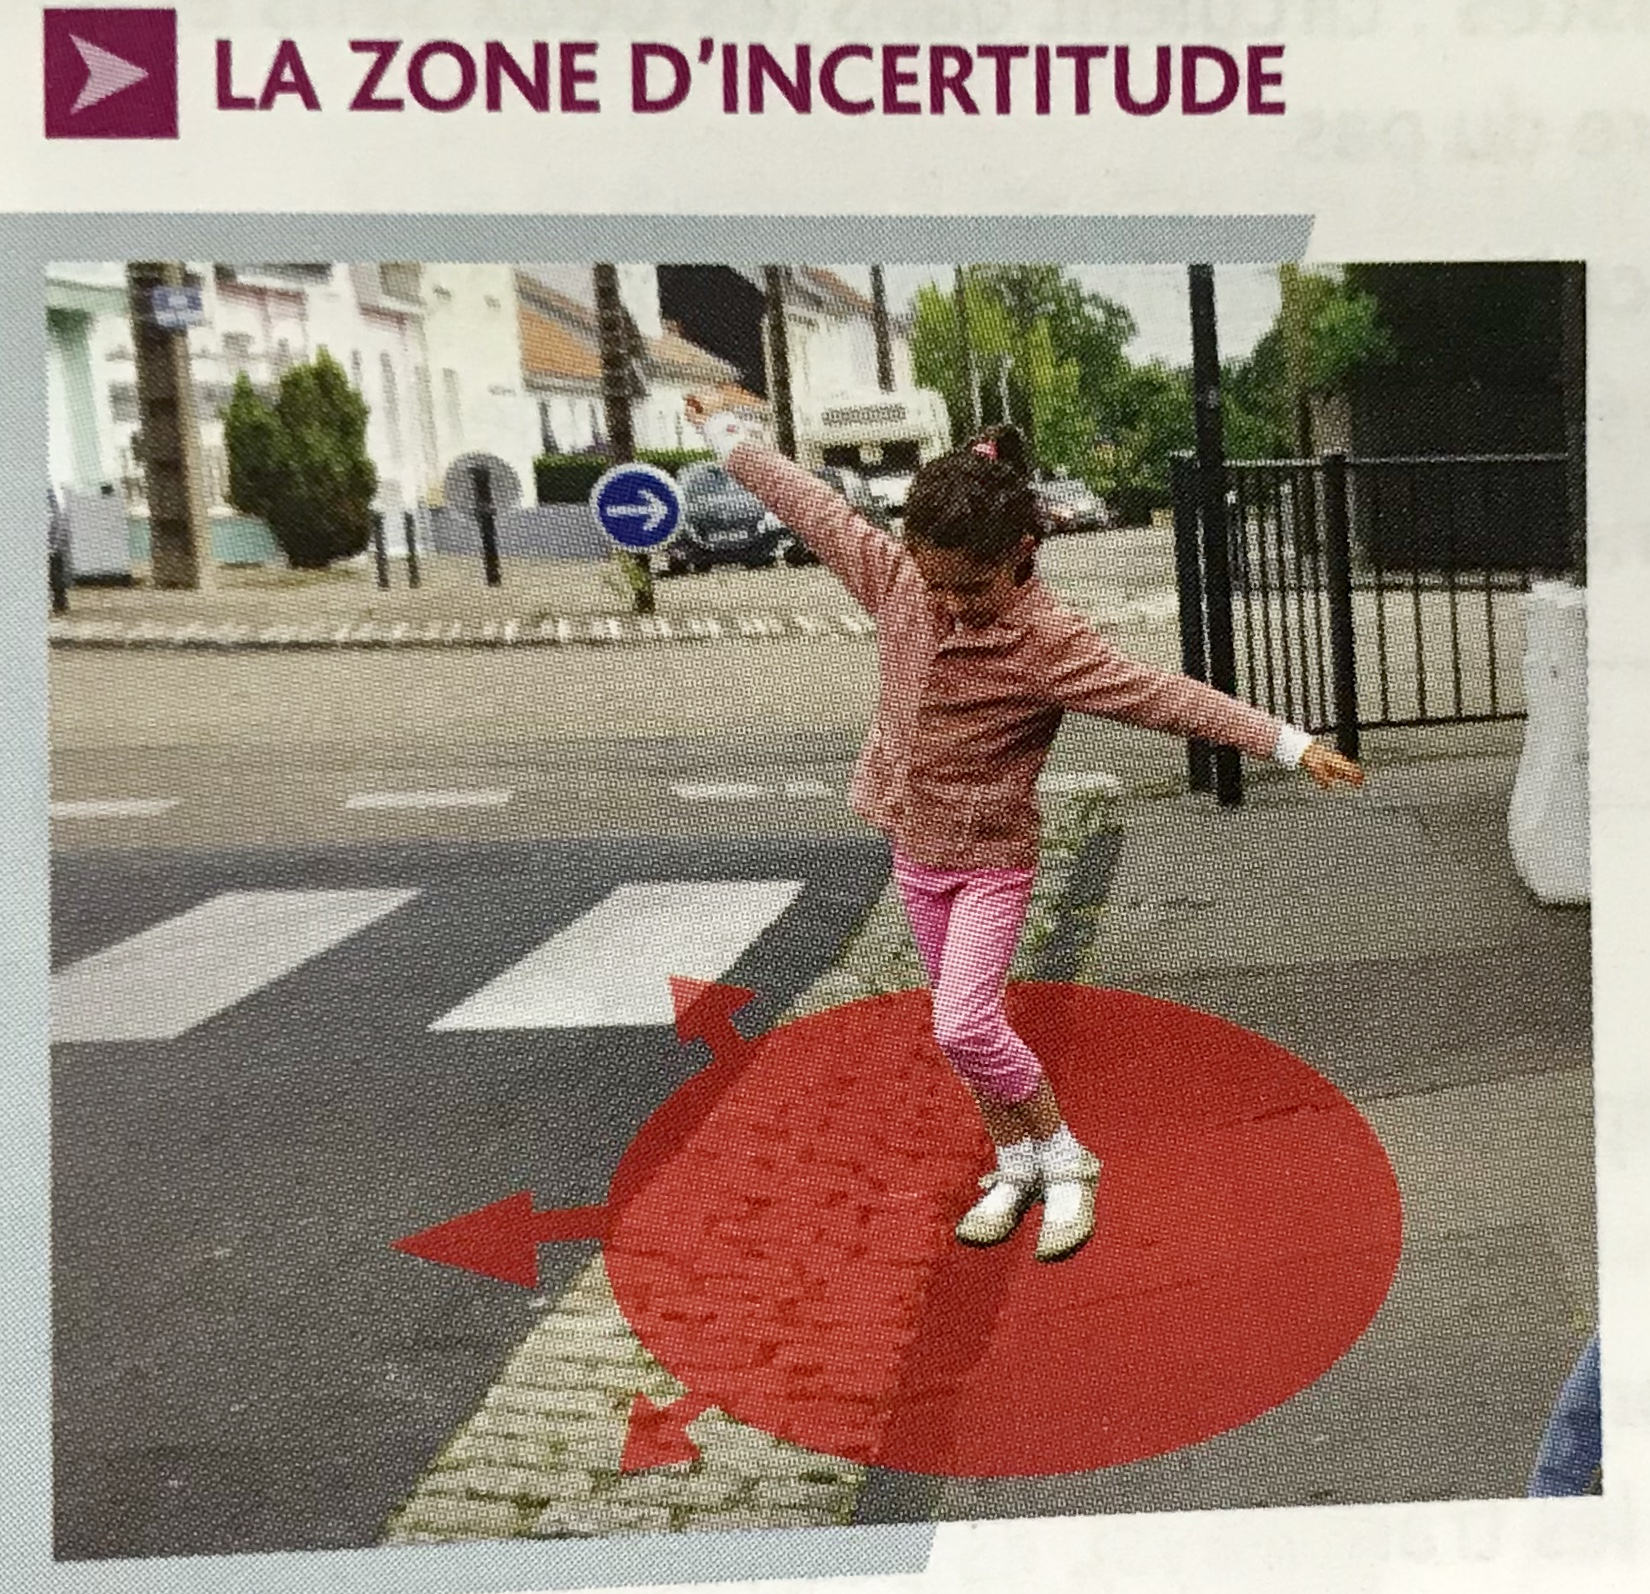
\includegraphics[width=\linewidth]{img/po-intentions}
		\caption{"Area of uncertainty". A partial observability stemming from unknown intentions of human agents.}
		\label{fig:po-intentions}
	\end{subfigure}
	\caption{Sources of Partial Observability in Autonomous Driving. Illustrations from \citep{ObjCode2017}.}
	\label{fig:partial-observability}
\end{figure}
\begin{figure}[th]
	\centering
	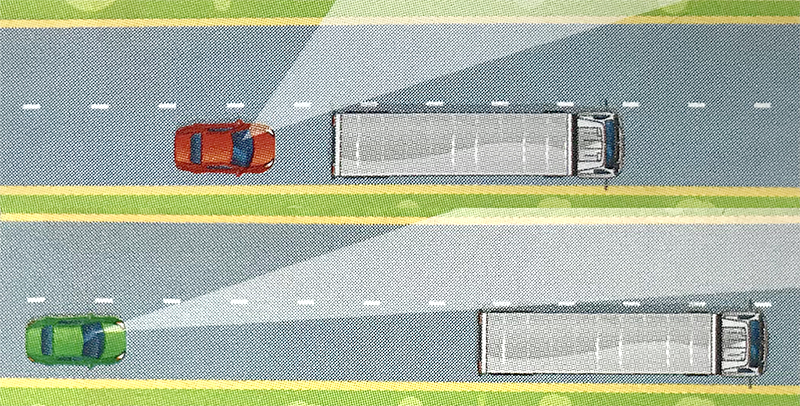
\includegraphics[width=0.7\linewidth]{img/pomdp}
	\caption{Information-seeking behaviours: the tailgating vehicle (top) should slow down, although it might decrease its immediate rewards, to gain valuable information in return (bottom). Image from \citep{ObjCode2017}.}
	\label{fig:information-seeking}
\end{figure}

In order to specify an \ac*{MDP}, the first step consists in defining the state space $\cS$, with the underlying assumption that the agent will have access to its current state $s\in\cS$. Yet in practice, information about the scene can only be obtained through sensors, which produce typically noisy measurements \citep{Ulbrich2013,Du2010}. Worse, parts of the state may be missing altogether, as is the case when a scene entity is occluded by an obstacle \citep[\eg][]{Brechtel2013,Bouton2018,Sun2019}, as shown in \Cref{fig:po-occlusion}. To account for these difficulties, the concept of a \emph{Partially Observable} Markov Decision Process (POMDP) was introduced in \citep{Astrom1965}, extending the MDP framework with two additional quantities: an observation space $\Omega$, and an measurement model $O$ such that the observation $o\in\Omega$ is measured at state $s'$ with the conditional probability $O\parentheses{o\mid s',a}$. At each time step $t$, a belief $b_t\in\cM(\cS)$ over the state $s_t\in \cS$ is updated by performing Bayesian Filtering to compute the posterior state distribution:
\begin{equation*}
b_{t+1}(s_{t+1}) = \frac{O(o_t|s_{t+1}, a_t)\sum_{s_{t}\in\cS}P\parentheses{s_{t+1} \mid s_t, a_t}b_t(s_t)}{\sum_{s\in\cS} O(o_t|s, a_t)\sum_{s_{t}\in\cS}P\parentheses{s \mid s_t, a_t}b_t(s_t)}.
\end{equation*}
By conditioning the policy $\pi(a_t|b_t)$ on the belief $b_t$, the POMDP framework allows to optimally balance between information gathering and task completion, as shown in \Cref{fig:information-seeking}. However, there is a price to pay: the belief space $\cM(\cS)$ is much larger than the state space $\cS$ (\eg continuous of dimension $n$ when $\cS$ is finite of size $n$), which drastically increases the planning complexity. Exact solutions exist when $\cS$ is finite \citep{Pineau2003}, and approximate ones when it is compact \citep{Porta2006,Silver2010}. Even the belief update is intractable in general, when $\cS$ is compact. In the case of linear dynamics and Gaussian measurement noise, the belief update is known as Kalman Filtering \citep{Kalman1960}. It has been applied in \citep[\eg]{Bry2011,Bouton2017,VanDenBerg2017}, and in the context of quadratic costs --\ie the standard LQG problem-- which enables efficient computation of the optimal policy \citep[see e.g.][]{Xu2014,VanDenBerg2011}. The more complex observation model of sensor occlusions in continuous-space is handled in \citep{Brechtel2013,Brechtel2014,Bouton2018} where cautious driving policies are learned for crossing intersections; and in \citep[][]{Sun2019} where the observed behaviour of nearby vehicles is used to infer the presence of potentially occluded pedestrians.
Furthermore, the POMDP framework has been used to account for uncertainty in the intentions of other agents, as illustrated in \Cref{fig:po-intentions}. In \citep{Bandyopadhyay2013}, the authors propose a Mixed-Observability framework (MOMDP) in which the other drivers locations are observed but not their destinations. In \citep{Barbier2018}, the uncertainty lies in whether the other agents intend to yield of take the right of way. The value of inferring these drivers intentions has been assessed in \citep{Sunberg2017}, in comparison to MDP baselines where a static or maximul-likelihood behavioural model is assumed instead.



\section{Actions and temporal abstraction}
\label{sec:temporal-abstraction}

\begin{figure}[th]
	\centering
	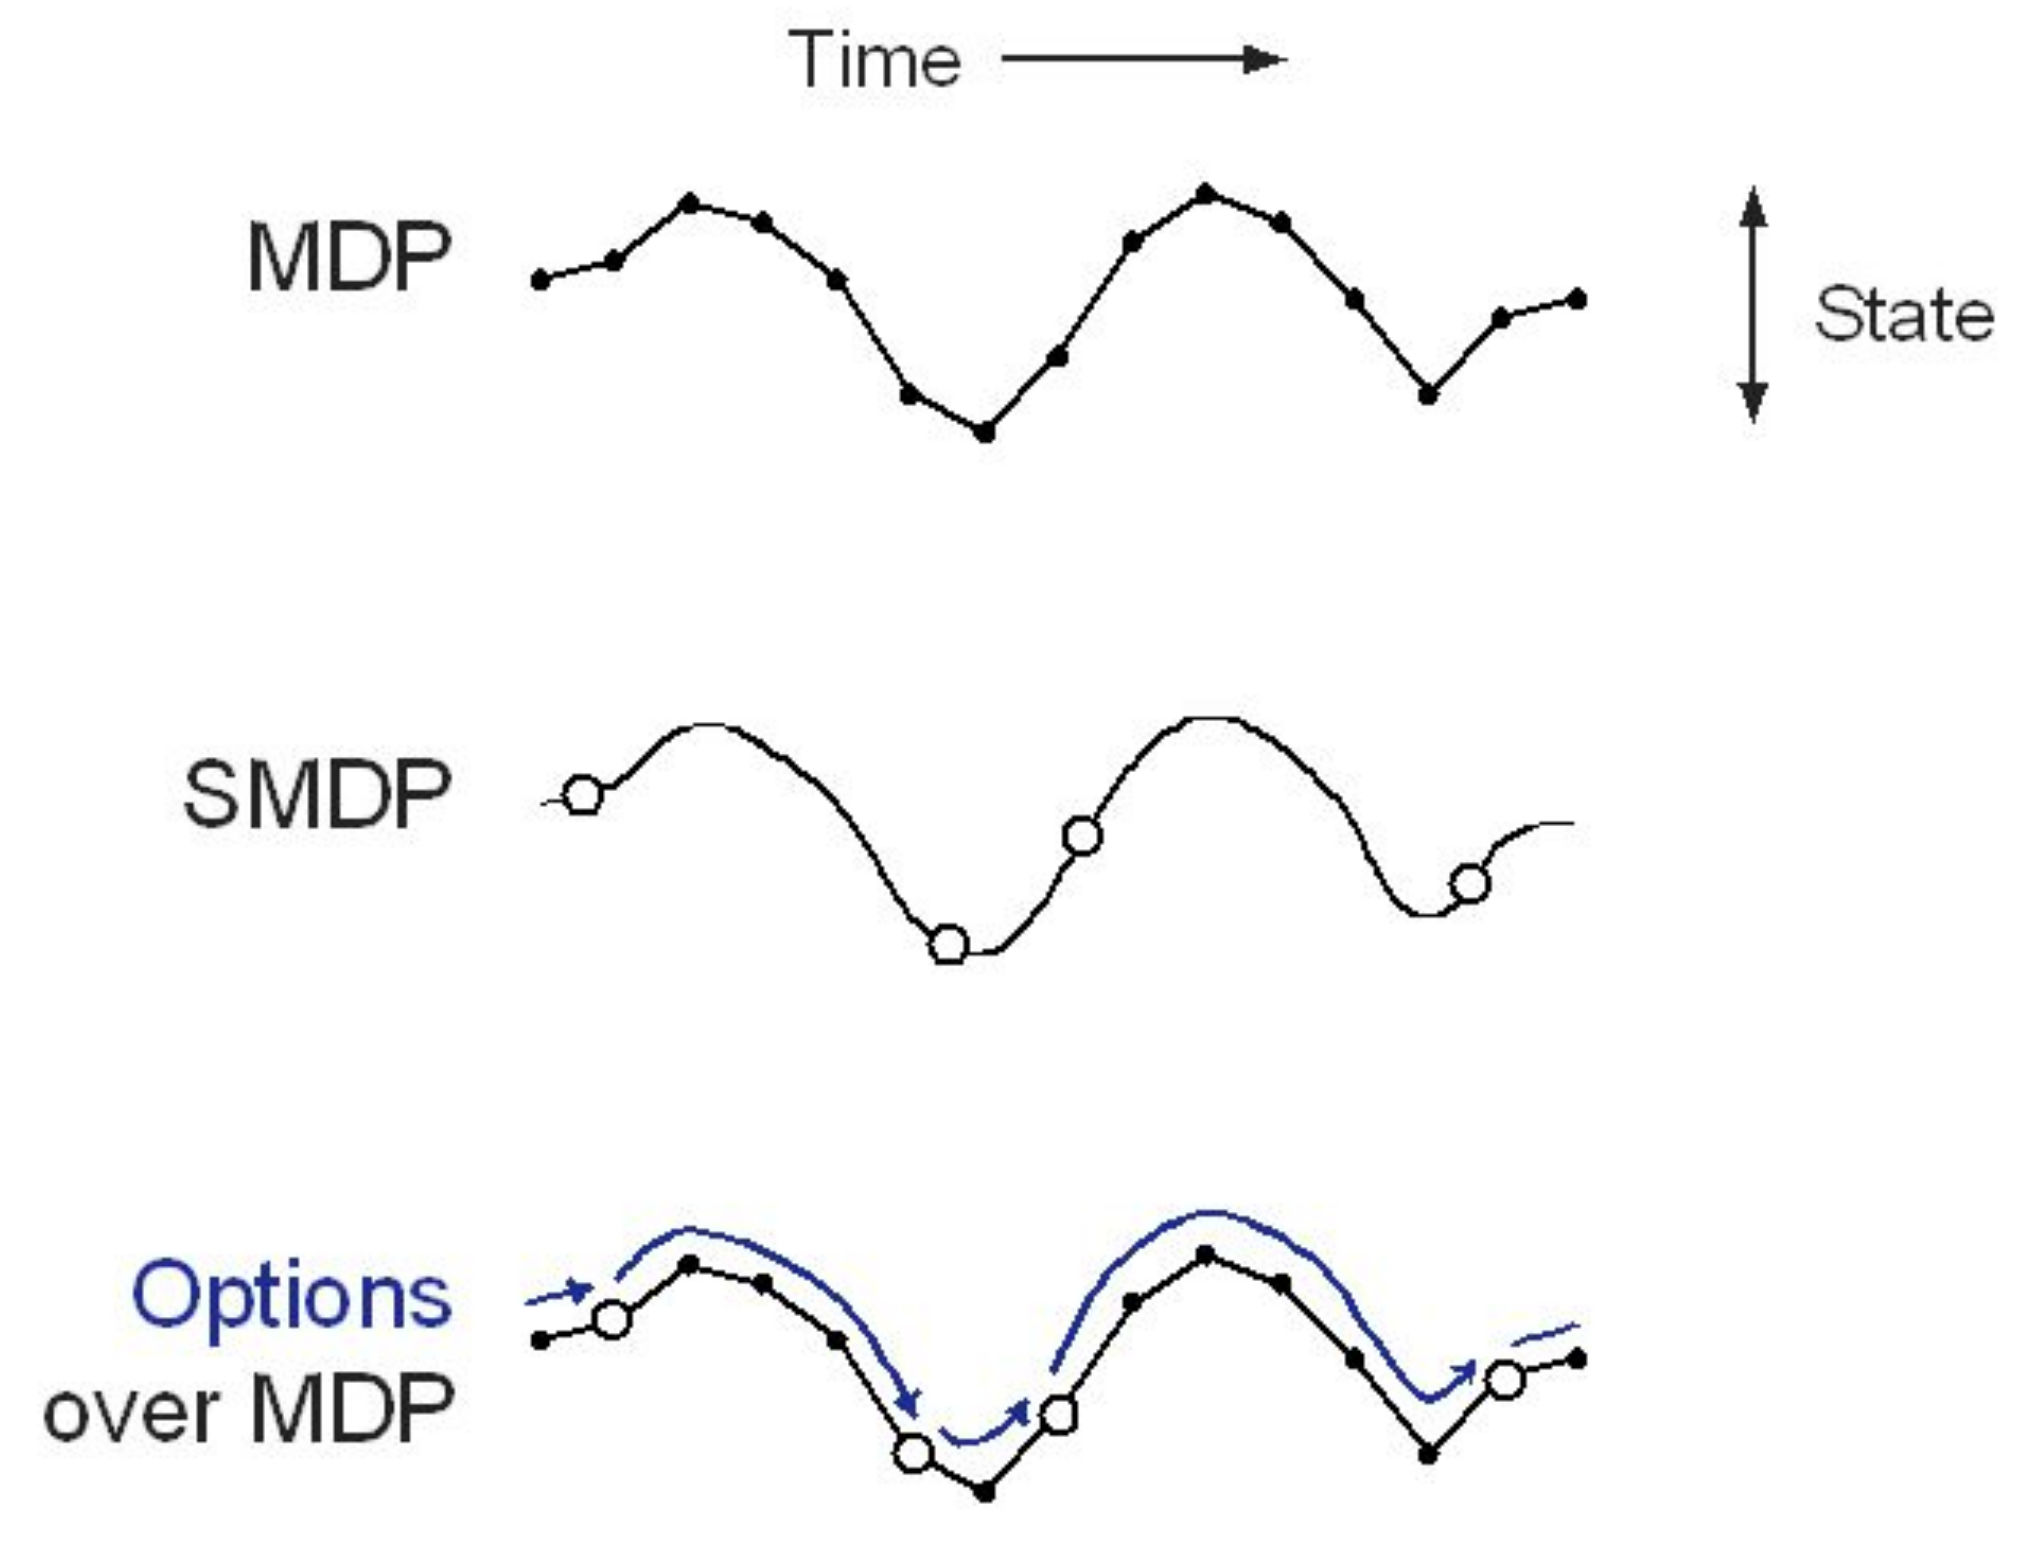
\includegraphics[width=0.5\linewidth]{img/smdp}
	\caption{Temporally extended sequences of actions can be used as skills, or \emph{options}, and futher used by a meta-policy to plan over long time horizons \citep{Sutton1999}.}
	\label{fig:smdp}
\end{figure}

The second step of when specifying an MDP is to choose an action space $\cA$. Suppose you are taking your first driving lesson, your instructor will be providing you with very detailed instructions about actuation such as: \emph{"turn the steering wheel by a full turn"}, \emph{"change gear"}, \emph{"brake smoothly"}, etc. After a few lessons however, the instructor will switch to more general instructions such as \emph{"change lane to overtake this vehicle"}, \emph{"yield to vehicles on the roundabout before merging"} or \emph{"drive slower in this area"}. And when, having finally got your driver's license, you start driving in an unfamiliar city, your friend in the passenger seat will merely give you directions: \emph{"follow the signs for the train station, and turn into the third street on the left"}. In short, driving involves reasoning at several time scales, and the corresponding decisions have different granularities. This can hardly be expressed in the MDP framework, where a single action space $\cA$ is considered. In particular, relying on shorter actions yields a smaller signal-to-noise ratio, which leads to slow learning when planning over long time horizon \citep{ShalevShwartz2017}. To address this issue, the concept of \emph{temporal abstraction} was introduced: nuclear actions $a\in\cA$ can be used to define temporally-extended \emph{skills} $\pi_o:\cS \rightarrow \cM(\cA)$, also called \emph{options}, which in turn can be used as meta-actions by a high-level \emph{option policy} $\pi(o|s)$. This idea is also referred to as \emph{Hierarchical Reinforcement Learning}, and was first analysed with the \emph{semi}-Markov Decision Process (SMDP) extension \citep{Sutton1999}, illustrated in \Cref{fig:smdp}. In autonomous driving, this hierarchy is typically imposed by the pipeline presented in \Cref{chapter:1}: Behavioural planning corresponds to the policy over options $\pi(o|s)$, while the low-level options $\pi_o$ are achieved in the Motion planning layer. However, this requires manually specifying the interfaces at each layer. For instance, in \citep{Barbier2018} a behavioural policy can only be trained after having defined a finite set of low-level skills, namely \emph{Stop}, \emph{Yield}, and \emph{Pass}. Consequently, using a fixed set of options constrains the comprehensiveness of the set of option-policies, and may prevent recovering optimality if the architecture is not versatile enough. To bypass these limitations, \citet{ShalevShwartz2016} proposed to ensure sufficient comprehensiveness of the class of available options by generating new options on-the-fly as paths in an option-graph, shown in \Cref{fig:options-graph}. Other works attempt to learn low-level skills jointly with the meta-policy \citep{Bacon2017,Vezhnevets2017,Heess2016}. In \citep{Paxton2017}, low-level skills such as \emph{follow} and \emph{overtake} are trained using Neural Networks and ad-hoc reward functions, while serving as meta-actions for a high-level tree-based planner.

\begin{figure}[th]
	\centering
	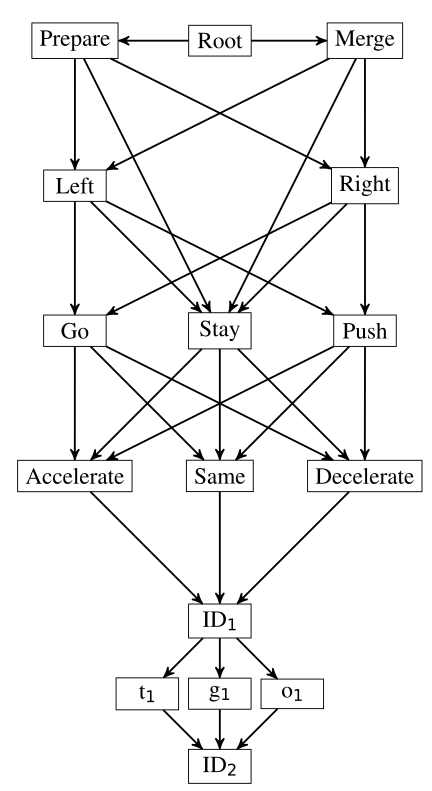
\includegraphics[width=0.3\linewidth]{img/options}
	\caption{A graph used to generate options \citep{ShalevShwartz2016}.}
	\label{fig:options-graph}
\end{figure}

\section{Rewards and inverse reinforcement learning}
\label{sec:irl}

Having defined the state and action spaces $\cS$ and $\cA$, we come to specify which state-action pairs are deemed \emph{desirable}, through the definition of the reward function $R$. Paradoxically enough, humans know how to drive but not necessarily how to explicit the reasons for their actions, especially in the form of a fixed evaluable objective. A common approach to reward specification is colloquially known as \emph{reward engineering}, in which the reward function is typically parametrized as a linear combination of features $R(s,a) = \sum_i \omega_i \phi_i(s,a)$ . For example, such features may include the ego-vehicle speed, its longitudinal distance to a short-term goal, lateral distance to the lane centerline, or the presence of collisions.
By handling more and more use-cases, the number of features to consider will rise quickly, some of which contradicting each other. Then, the issue of how the properly choose the weights $\omega_i$ remains, and it can be increasingly hard to strike the right trade-off.
Besides, this difficulty is further exacerbated by an ambiguity lying in the blurry boundary between the reward function $R(s,a)$ and the value function $V(s)$. For instance, are safety distances desirable \textit{per se}, or only because respecting them means we are less likely to end up in an accident, which is the actual feature of interest here? Likewise, do road traffic regulation rules describe rewarding states or high-value states?

\begin{figure}[ht]
	\centering
	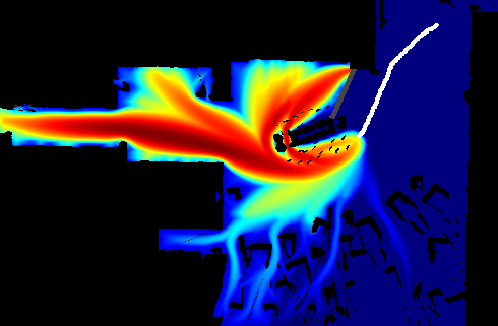
\includegraphics[width=0.6\linewidth]{img/pedestrian}
	\caption{Trajectory prediction for a pedestrian modelled as an optimal planner with a learned cost \citep{Ziebart2009}.}
	\label{fig:irl-pedestrian}
\end{figure}


One practical solution to these concerns is to iteratively refine the reward function $R$ until the corresponding optimal policy $\pi^\star$ matches the expected behaviour $\pi_E$ of human drivers. The careful or well-versed reader will have noticed that this approach is directly opposed to the \acl*{RL} problem, where the optimal behaviour $\pi^*$ stems from the reward function $R$. Accordingly, the aptly named \ac{IRL} framework aims at finding a reward function that makes the expert behaviour appear uniquely (near)-optimal. At first glance, this problem seems related to Imitation Learning formulation of \Cref{sec:imitation-learning} in its attempt to reproduce expert behaviour. This intuition is supported by the fact that \ac{RL} $\circ$ \ac{IRL} is the dual problem of state-action occupancy matching with respect to expert trajectories \citep{Ho2016}. Example applications of \ac*{IRL} to \acl*{AD} include the work of \citet{Kuderer2015} who learn the trade-off between comfort and efficacy in human lane-change trajectories. 

In addition to finding a good candidate reward for the ego-vehicle behaviour, \acl*{IRL} can also be applied for the purpose of predicting how other agents in the scenes are likely to behave, by modelling them as rational agents trying to maximise an unknown reward function to be learned. In that sense, \ac{RL} $\circ$ \ac{IRL} is a form of model-based \acl*{RL}.
For instance, this approach has been used to model of routing preferences of taxi-drivers \citep{Ziebart2008}, to predict the future trajectory of pedestrians \citep{Ziebart2009} as shown in \Cref{fig:irl-pedestrian}, and the behaviour of human drivers at an intersection \citep{Sun2019} or on a highway \citep{Sadigh2016}.


\section{Dynamics, offline learning and transfer}

We now come to the last element of the \acl*{MDP} tuple: the dynamics $P\parentheses{s'\mid s,a}$. Contrary to the state and actions which are the input and output interfaces of the agent, and to the reward function which is generally chosen by the system designer, there is usually no need to actually specify the system dynamics. Indeed, one of the biggest assets of Reinforcement Learning is its ability to handle unknown dynamics that are only accessed through interaction. Unfortunately, this assumption that the agent is allowed direct interaction with true environment is both unacceptable and unrealistic in the context of \acl*{AD}. Indeed, the traditional \emph{learning-by-acting} pipeline requires exploration, which would imply having autonomous vehicles violate the rules of the road and generate accidents, which is obviously out of question. Besides, most \acl*{RL} algorithms require a tremendous amount of interaction data to learn an optimal policy, including for \acp*{MDP} such as Atari games which are arguably less diverse and complex than real-world driving scenes. Not to mention that, perhaps evidently but contrary to simulated games, \emph{the real world can only run in real time}.

This issue can be addressed in two ways. A first solution is to consider the \emph{offline} \acl*{RL} problem \citep{levine2020offline}, in which the agent no longer has the ability to interact with the environment and is instead provided with a \emph{static} dataset $\cD = \{(s_t, a_t, r_t, s_{t+1})\}$ of interaction data, and must learn the best policy it can with this dataset. These interaction data that are collected by an exploration policy $\pi_E$, in our case human driving. However, for the same reasons mentioned in \Cref{sec:imitation-learning}, this limited data available induces a loss of optimality: any attempt to improve the policy may steer the agent in regions of the state space $\cS$ that are not present in the dataset $\cD$, typically accident states, off-road driving, \etc in the case of \acl*{AD}. Still, safe policy improvement guarantees can be derived under some conditions, \eg for finite \acp*{MDP} \citep{Laroche2019,Nadjahi2019}. This often requires to constrain how much the learned policy $\pi$ can differ from the exploration policy $\pi_E$, so as to bound the state distribution shift \citep{Kakade2002,Schulman2015}.

\begin{figure}[ht]
	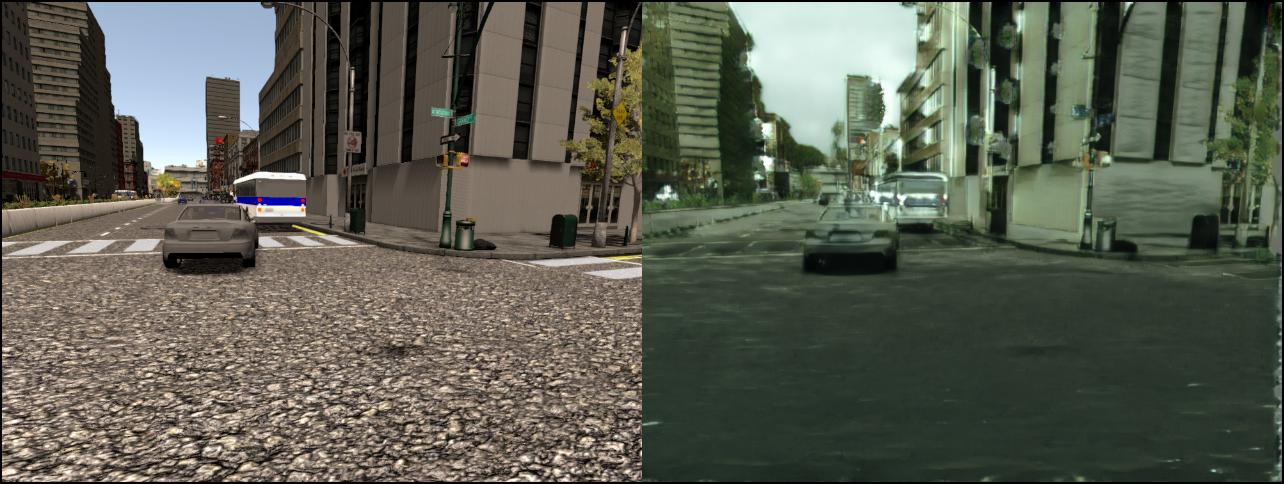
\includegraphics[width=\linewidth]{img/transfer}
	\caption{Sim-to-real unsupervised transfer \citep{Liu2017} from synthetic images of the \textsc{cynthia} dataset \citep{Ros2016} to realistic images of the \textsc{Cityscapes} dataset \citep{Cordts2016}.}
	\label{fig:transfer}
\end{figure}

A second decision is to leverage \emph{simulation}. The vast majority of \acl*{RL} systems currently running are interacting simulated environments. Indeed, simulation provides many advantages: it is generally much cheaper than real experiments, it can run much faster, be easily parallelised, be reset to any initial state when it fails, and failures are not costly and can be experienced at will. Unfortunately, all these benefits come at a price: there is always a \emph{gap} between simulation and reality, an issue also known as \emph{model bias}. The problem of adapting a policy learned in one environment to another related one is known as \emph{Transfer}, and has been tackled by researchers in different ways. A general strategy is to use simulation as a pre-training and fine-tune to the policy in the target environment \citep{Liang2019}. This allows to obtain satisfactory initial behaviour and cut down on training time. To reduce the gap between the simulation and reality, three approaches can be taken:
\begin{enumerate}[label=(\roman*)]
	\item make the simulation as \textit{realistic} as possible. For instance, \citet{Pan2017} translate the virtual images rendered by a simulator to synthetic realistic images, using an Image-to-Image Translation Networks similar to that shown in \Cref{fig:transfer}, so that the observations seen by the agent while training at closer to those it will observe when deployed in the real environment.
	\item make the simulation more \textit{diverse}, by partially randomizing the observations and dynamics, so that the real world appears like yet another realization of that diversity. This approach is known as \emph{Domain Randomization}, and has been widely applied to robotic manipulation tasks \citep{Tobin2017,openai2019solving}, and in the context of \acl*{AD} \citep{Prakash2019,Pouyanfar2019}.
	\item make both the simulation and the real-world \textit{abstract}, by mapping them to intermediate observation and action spaces so that the encapsulated policy is not directly exposed to raw perceptual inputs and low-level controls. For instance, semantically segmented images and waypoints are used as observations and actions in \citep{Mueller2018}.
\end{enumerate}


\section{Optimality criterion and safety}


\begin{figure}[ht]
	\centering
	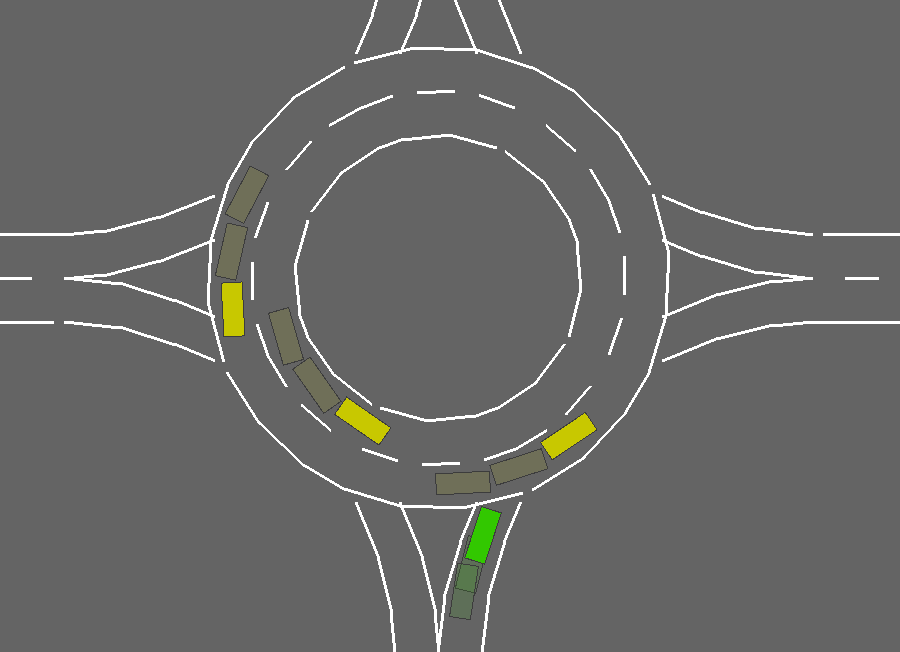
\includegraphics[trim={0 0.5cm 0 0}, clip, width=0.5\linewidth]{img/roundabout3-small}
	\caption{A risky situation: should the vehicle merge into the roundabout?}
	\label{fig:risky-problem}
\end{figure}
\begin{table}[ht]
	\centering
	\begin{tabular}{lccc}
		\toprule
		Decision & \multicolumn{2}{c}{Merge} & Wait \\
		\cmidrule(lr){2-3}
		\cmidrule(lr){4-4}
		Outcome & Success & Failure & Boredom \\
		Probability & $1-\delta$ & $\delta$ & 1 \\
		Reward & $1$ & $-\frac{1-\delta}{\delta}$ & 0 \\
		\midrule
		$\expectedvalue[R]$ & \multicolumn{2}{c}{$0$} & $0$ \\
		$\mathop{\mathbb{V}}(R)$ & \multicolumn{2}{c}{$\frac{1-\delta}{\delta} \simeq \frac{1}{\delta}$} & $0$ \\
		$\min R$ & \multicolumn{2}{c}{$-\frac{1-\delta}{\delta} \simeq -\frac{1}{\delta}$} & $0$ \\
		\bottomrule	
	\end{tabular}
	\caption{A simple bandit problem associated with \Cref{fig:risky-problem}. When trying to merge, an accident happens with probability $\delta$ and the agent suffers a high penalty $\frac{1-\delta}{\delta}$. If the agent decides to wait instead, it suffers a small penalty of $0$ for the inconvenience. We show the associated expected reward, worst-case reward, and reward variance.}
	\label{tab:risky-problem}
\end{table}

Once the \acl*{MDP} is fully specified, a policy $\pi$ is said to be optimal if it maximises the \emph{expected} return
\begin{equation*}
\max_\pi \expectedvalue_{\pi, P} \left[\sum_t \gamma^t R_t \right].
\end{equation*}

But is this an appropriate performance measure? Consider a driving decision --say merging into a roundabout as illustrated in \Cref{fig:risky-problem}-- that, given the uncertainty on the behaviour of other agents, can lead to a collision with a certain probability $\delta$. When maximising the return in expectation, the agent is allowed balance the rare accident penalty with the more likely perspective of a successful merge. As observed by \citet{ShalevShwartz2017}, assuming that rewards are normalized in $[0, 1]$ for standard behaviours, for the agent to care about avoiding accidents with probability $1-\delta$ requires the penalty associated with a collision to be in order of $1/\delta$, as we illustrate in \Cref{tab:risky-problem}. This leads to a high variance in the observed rewards, which is likely to impede learning. 
Furthermore, the optimal agent is willing to gamble a collision now and then, if it allows for an increased efficiency the rest of the time. This question of whether and how to weigh human lives with economical benefits brings us straight back to the ethical considerations of \Cref{sec:trolley}.

This questioning has lead researchers and practitioners to consider alternative definitions of optimality, tailored for an increased awareness of events of small probability and high consequences. These approaches are grouped under the name of \emph{Safe} \acl*{RL}, and typically involve giving up some expected performance in favour of the lower tail of the return distribution. They were surveyed by \citet{Garcia2015}, who identified four main paradigms: the first three involve a change of the optimisation criterion, while the fourth one defines a constraint on the exploration process.

\subsection{Risk-sensitive Criterion}

Risk-sensitive methods augment the traditional expected performance criterion with a measure of \textit{variability}. For instance, in the above example of \Cref{tab:risky-problem} the two decisions are equivalent in terms of expected return, but \texttt{Merge} has a significantly higher variance than \texttt{Wait}.  A first instance of risk-sensitive objective is the \emph{variance-penalized} criterion \citep{Markowitz59} with weight $\alpha > 0$, which takes the form:
\begin{equation*}
\max_\pi \expectedvalue_{\pi, P} \left[\sum_t \gamma^t R_t\right] - \alpha\mathop{\mathbb{V}}_{\pi, P} \left[\sum_t \gamma^t R_t \right].
\end{equation*}

Many other risk measures have been investigated such as the \ac{VaR}, the \ac{CVaR} and percentile performance, in both the \acl*{MAB} setting \citet{Torossian19a} and the \acl*{RL} setting \citep{Moody2001,Tamar2012,Prashanth2013,Delage2010}. In their seminal paper, \citet{Artzner1999} identified a set of properties deemed necessary for a risk measure to be \emph{coherent}, and policy gradient methods have been designed to optimise this class of measures \citep{Tamar2015}.
In the context of \acl*{AD}, the variance-penalised objective has been applied in \eg \citep{Naghshvar2018} to highway ramp scenarios with occlusions and limited sensor range.

\subsection{Worst-case criterion}

In model-based \acl*{RL}, the model parameters are typically estimated from noisy interaction data, which can lead to modelling errors that may have fatal consequences in real, physical systems. To address this issue, robust control community has formulated to optimise the outcome of a policy $\pi$ with respect to an \emph{ambiguity set} $\cP$ of likely dynamics:

\begin{equation*}
\max_\pi \min_{P\in\cP} \expectedvalue_{\pi, P} \left[\sum_t \gamma^t R_t\right]
\end{equation*}

This problem was first studied by the control community, who focused on the minimax control of the $\cH_\infty$-norm \citep[][]{Basar1996} and $\cH_2$-norm \citep{Berkenkamp2015} of linear systems. Minimax-control of quadratic costs --the so-called robust \ac{LQ} problem-- was later considered in \citep{abbasi-yadkori11a,Ibrahimi2013,Faradonbeh2017,Ouyang2017,abeille18a,Dean2017,Dean2018}.
The case of finite \acp*{MDP} with uncertain parameters was studied by \citet{Iyengar2005,Nilim2005,Wiesemann2013}, who showed that the main results of \ac{DP} could be recovered under a \emph{rectangularity} assumption for the structure of uncertainty. Their work was extended to the \ac*{RL} setting in \citep{Tamar2014}.

%In the context of \acl*{AD}, \citep{Williams2018} used TubeMPC for driving.

\subsection{Constrained Criterion}
\label{sec:constrained-criterion}

Another approach is to formulate safety as constrained optimisation: the task is to maximise a target function $f(x)$ while satisfying an inequality constraint $g(x)\leq \beta$. For instance, \citet{Berkenkamp2016} apply this principle to safe blackbox optimisation using Gaussian Process regression. This idea is extended to a sequential decision-making in the \ac{CMDP} framework \citep{Altman1999,Achiam2017}, a variant of \acp*{MDP} augmented with a cost function $C$, and such that the return maximisation objective is subjected to a constraint on the maximum expected cumulative discounted cost:

\begin{equation*}
\max_\pi \expectedvalue_{\pi, P} \left[\sum_t \gamma^t R_t \right] \text{ subject to } \expectedvalue_{\pi, P} \left[\sum_t \gamma^t C_t \right] \leq \beta.
\end{equation*}

Extensions have also been proposed to this framework: in \citep{Tessler2019}, more general constraints than discounted sums are considered, while in \citep{Geibel2005,Chow2018} the constraint does concern the expectation of the discounted total cost, but rather its percentile or \ac{CVaR}. 
\acp*{CMDP} have been applied in \citep{Bouton2019workshop,Bouton2019} to control the probability for the ego-vehicle to reach its goal safely, and in \citep{Le2019} to enforce two behavioural constraints in car racing simulation: smooth driving (expected number of braking actions) and lane tracking (expected distance to the lane center).

\subsection{Safe Exploration}

The three paradigms mentioned so far aim to revisit the definition of optimality. However, these adjustments only alter the optimal policy once it is learnt, but they leave the exploration process subject to failures. Consequently, other approaches have been developed to enforce safety constraints at all time. The most common formalisation, robust constraint satisfaction, consists in preventing the agent from visiting any \emph{error state} during exploration --or equivalently to remain within a safe set $\mathbb{X}$-- by relying on prior knowledge such as expert demonstrations or an initial feasible policy.
According to \citet{Fraichard2014}, this objective is challenging as it requires the ability to \textit{"reason about the future"} as illustrated in \Cref{fig:ics-1}, and to \textit{"consider obstacles globally and not individually"} as shown in \Cref{fig:ics-2}.

\begin{figure}[ht]
	\begin{subfigure}[b]{0.48\linewidth}
		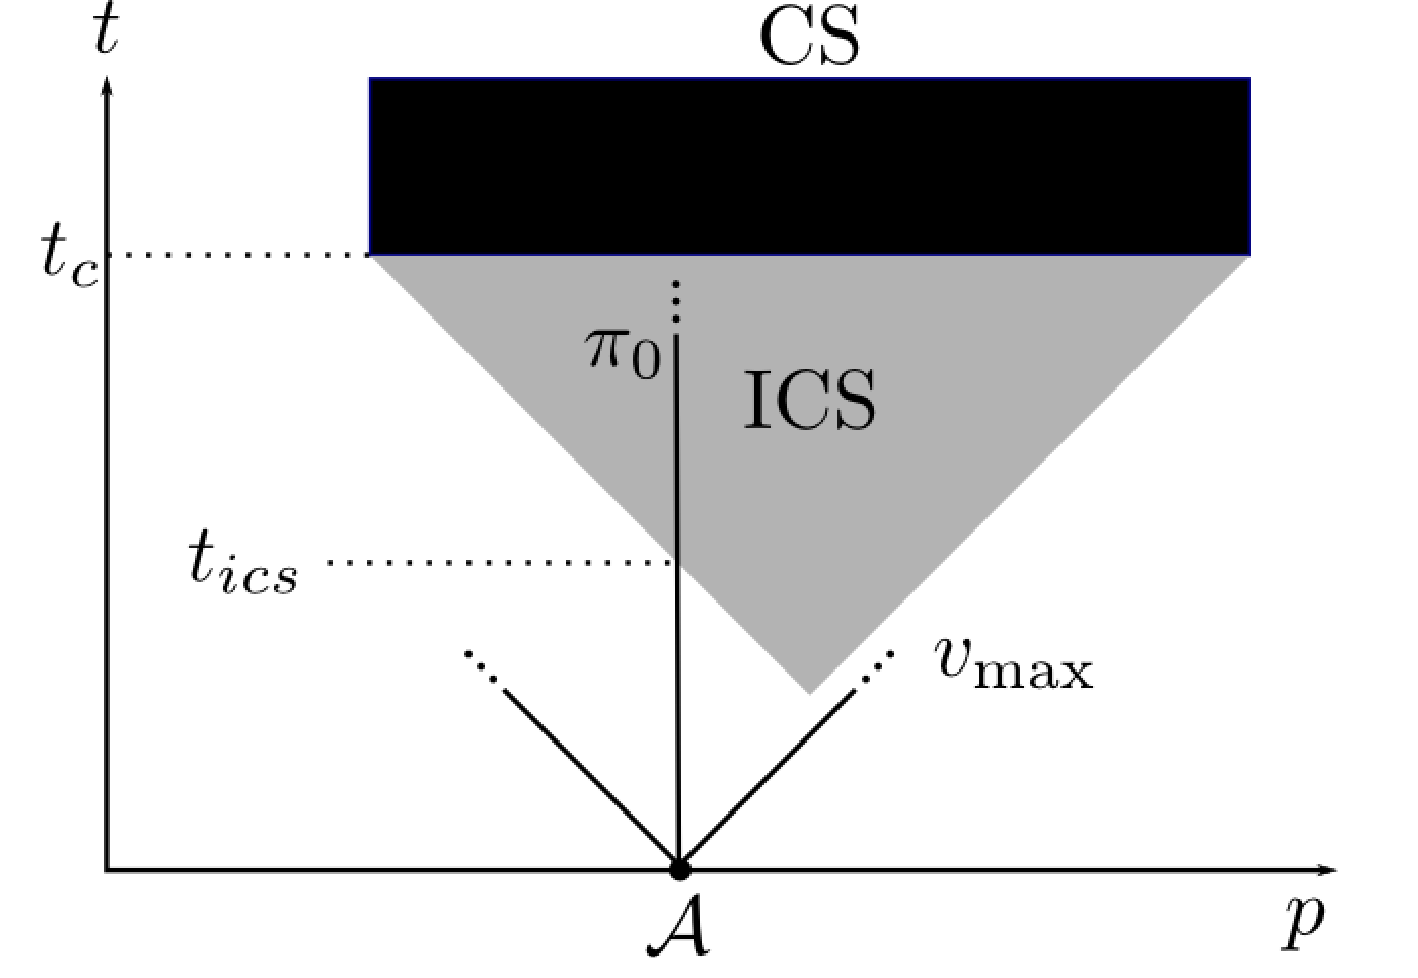
\includegraphics[width=\linewidth]{img/ics}
		\caption{A minimum horizon $T > t_c - t_{ics}$ is required}
		\label{fig:ics-1}
	\end{subfigure}
	\begin{subfigure}[b]{0.48\linewidth}
		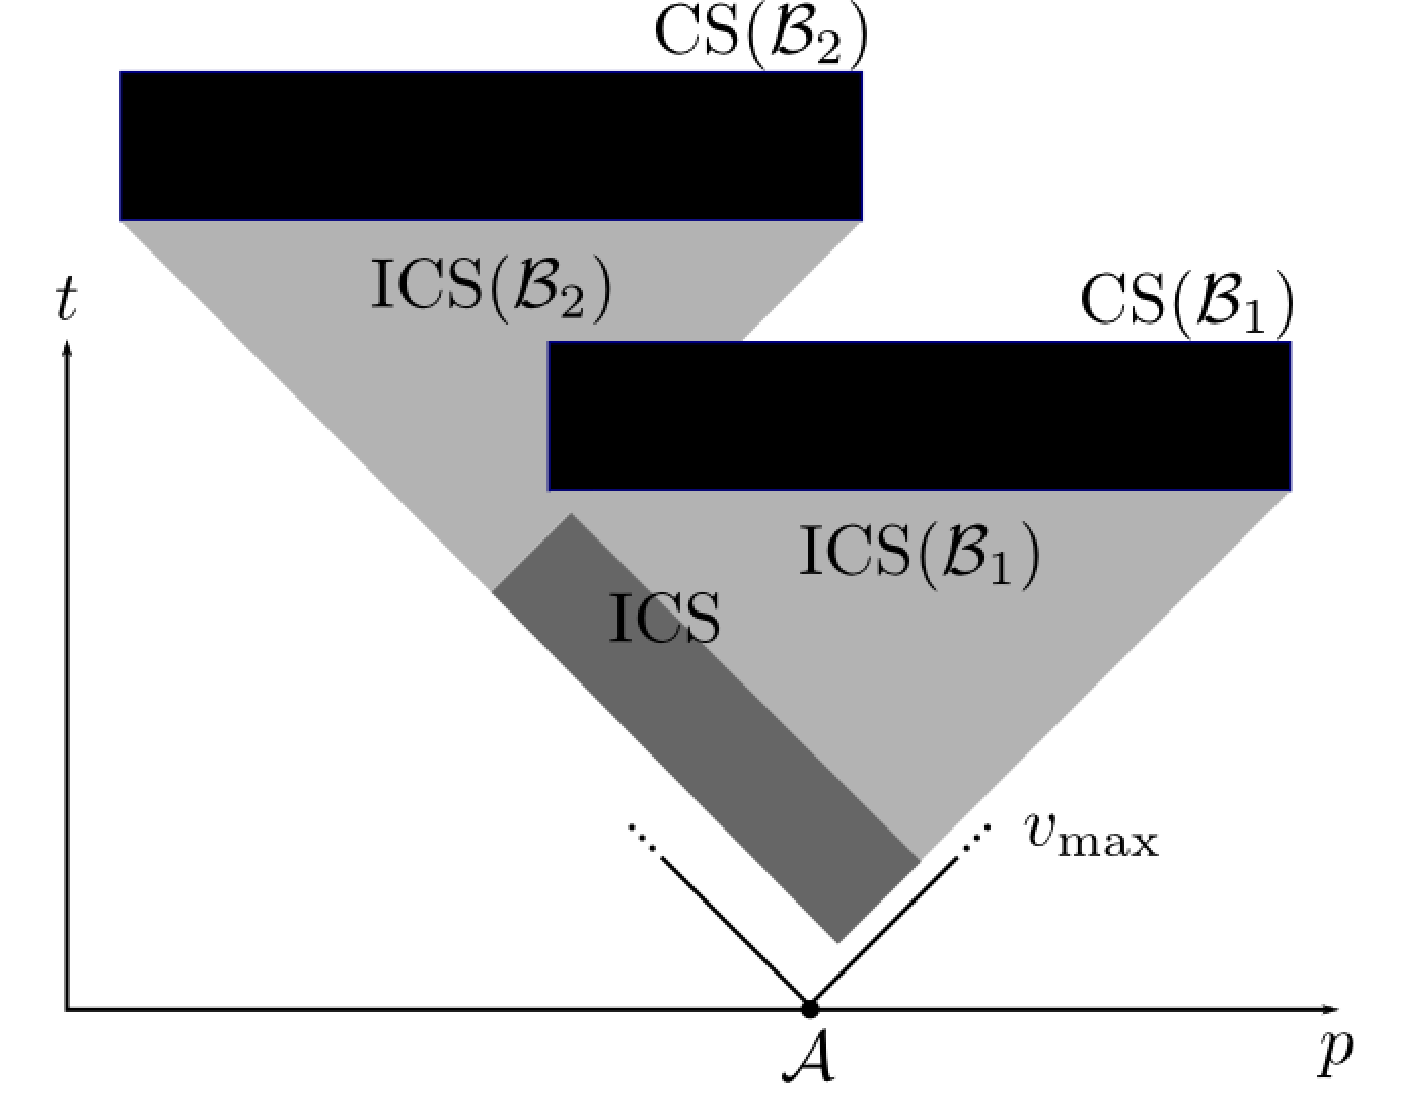
\includegraphics[width=\linewidth]{img/ics-global}
		\caption{Obstacles must be considered \emph{globally}.}
		\label{fig:ics-2}
	\end{subfigure}
	\caption{Inevitable Collision States (ICS), images from \citep{Fraichard2014}.}
	\label{fig:ics}
\end{figure}

When the system is fully known, a general solution to this problem is provided by the \ac{HJI} reachability equation, in the form of a differential game. This approach is followed in \citep{leung2018infusing,Fisac2019} by decomposing the system into a known deterministic part subject to an adversarial bounded perturbation. In the context of finite \acp*{MDP} with unknown dynamics, 
assuming the safe states are defined as the level-set of a safety function  $C(s,a) \leq \beta$ whose smoothness is known, \citet{Turchetta2016} propose an algorithm that explores a maximum \emph{reachable ergodic safe set} without visiting unsafe states.
Since solving the \ac*{HJI} equation is intractable in general, researchers have considered more structured special cases, namely linear systems and convex (often polytopic) constraints \citep{Fukushima2007,Adetola2009,Aswani2013,Lorenzen2017,Kohler2019,Lu2019}.

\begin{figure}[ht]
	\centering
	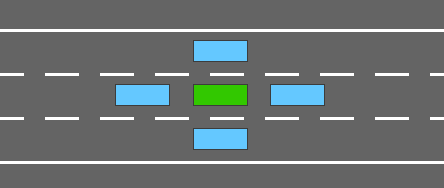
\includegraphics[width=0.45\linewidth]{img/safety_no_2_small}
	\caption{An ordinary highway-driving situation, but prone to accidents under adversarial behaviours.}
	\label{fig:no-safety}
\end{figure}
Yet, it is questionable whether the property of robust constraint satisfaction under adversarial disturbances is relevant for an \acl*{AD} application. Indeed, this requirement might be too restrictive since many nominal states are prone to errors under adversarial behaviours, as shown in the example of \Cref{fig:no-safety}. A strategy of avoiding this region of the state-space altogether would be overly cautious and unacceptable. To cope with that issue, weaker models of safety have been proposed. Thus, rather than avoiding all collisions, \emph{Passive} motion safety \citep{Macek2009,Bouraine2012,Bouraine2014} only requires the robot to be motionless whenever a collision could possibly occur. To account for limited dynamic capabilities of other agents, the stronger \emph{Passive-friendly} motion safety model was introduced \citep{Mitsch2017}, ensuring not only that the ego-vehicle safely stops itself, but also allows sufficient space for other vehicles to stop before a collision occurs. Note that this is equivalent to the original motion safety model with a restricted set of adversarial behaviours for other agents, requiring them to brake and avoid collisions when possible. Finally, \citet{ShalevShwartz2017} defines a notion of \emph{Responsibility Sensitive Safety} specific to \acl*{AD}, which formalizes \emph{"an interpretation of \emph{Duty of Care} from Tort law"}. This interpretation is summarized by five main rules tailored for a specific set of use-cases (including several road geometries, right of way rules, pedestrians and occlusions) and implemented as a set of dynamic geometrical constraints.

